

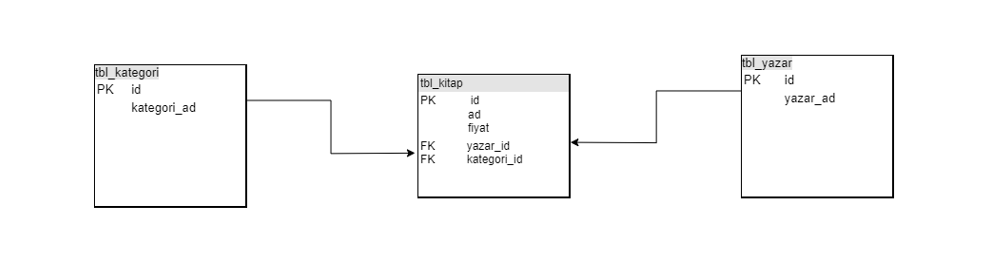
\includegraphics[ width=\textwidth]{tablolar.png} \newline



Database katmanında PostgreSQL'i tercih etmemin sebebi PostgreSQL'in açık kaynaklı yapısı ve lisans ücreti gerektirmemesi gibi avantajlarının olmasıdır.Çekirdek başına ve sürümüne göre maliyet diğer dillerde oldukça fazladır. PostgreSQL ile projede temel verileri depolamak için kullanılacak olan "kitap," "kategori," ve "yazar" gibi tabloları içermektedir.
Database işlemlerinde verinin kullanabilmesi için PostgreSQL fonksiyonlarından yararlanacağım.
\vspace{1\baselineskip} %
\newline

	PostgreSql fonksiyonları ile ilgili araştırmaları [\url{https://github.com/tubitak-bilgem-yte/pg-gelistirici.git}] adresinden gerçekleştirdim.\newline 
	
	\centering
	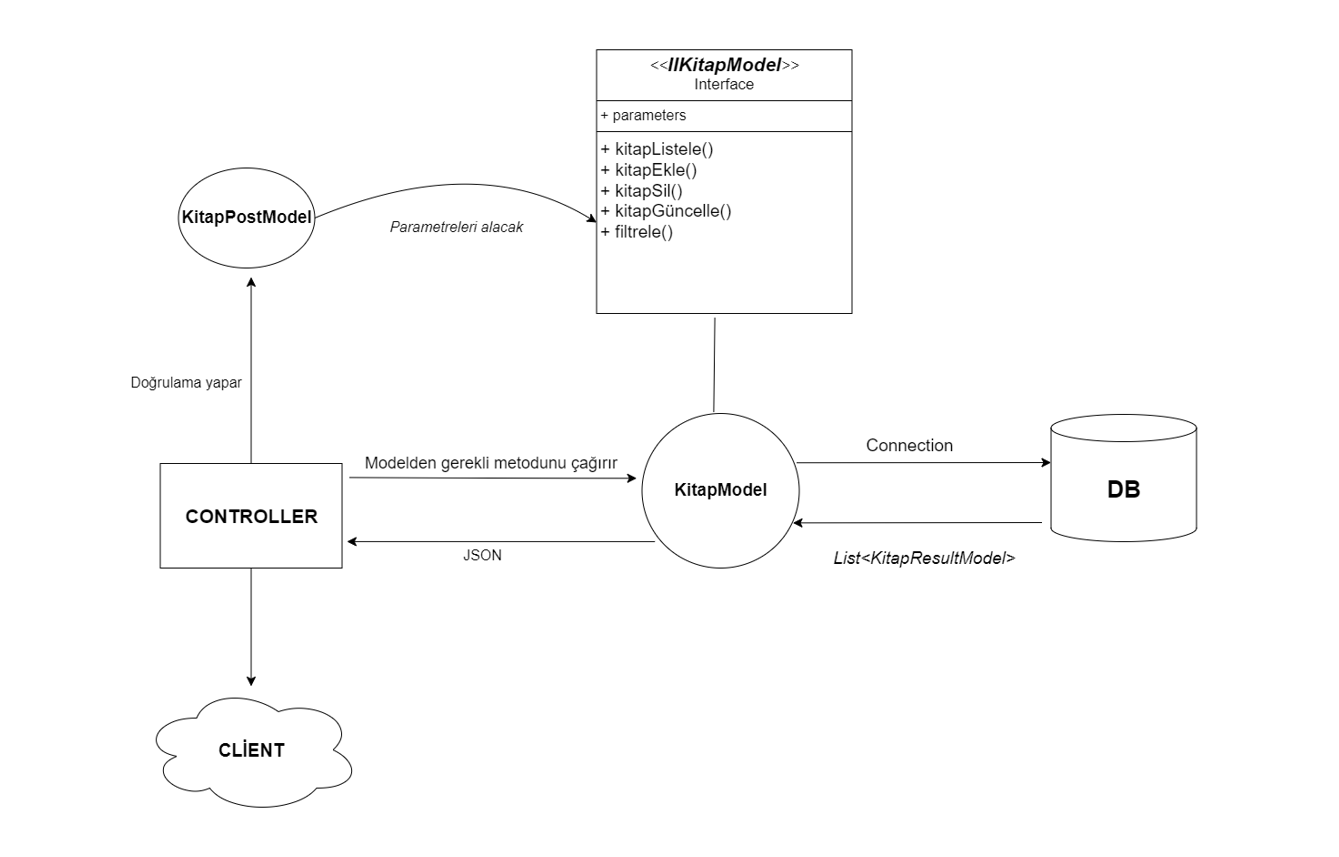
\includegraphics[ width=15cm, height=15cm,keepaspectratio]{Model.png} \newline


\begin{description}
	\item[\textbf{IKitapModel Arayüzü:}] Bu arayüz, kitaplarla ilgili işlemlerin sözleşmesini tanımlar. Yani, kitap listeleme ve kitap ekleme vb. işlevlerin prototiplerini içerir.Yapılacak işlemler için gerekli parametreleri KitapPostModel'den alır ve sonuç olarak bir KitapResultModel listesi döndürür.
	\item[\textbf{KitapModel Sınıfı:}] IKitapModel arayüzünü uygular (implement eder) ve bu arayüzde tanımlanan metodların somut davranışlarını içerir.
	PostgreSQL veritabanına bağlanır, bir SQL sorgusu çalıştırır ve sonuçları bir KitapResultModel listesine dönüştürür.
	Veritabanı bağlantısı ve sorgu işlemleri için NpgsqlConnection ve NpgsqlCommand nesnelerini kullanır.
	\item[\textbf{ KitapPostModel Sınıfı:}] Kullanıcıdan alınan verileri taşımak için kullanılır. Bu model,örneğin kitap listeleme işlemi sırasında kullanıcı tarafından sağlanan verileri (örneğin, bir kitap adı) içerir.
	\item[\textbf{KitapResultModel Sınıfı:}] Veritabanından dönen sonuçları temsil eder. Her bir KitapResultModel nesnesi, bir kitap kaydının id, ad, fiyat, yazarAd, kategoriAd gibi özelliklerini içerir.
	\item[\textbf{HomeController Sınıfı:}] MVC'nin Controller bileşenidir ve kullanıcı isteklerini yönetir.
	Index metodu, uygulamanın ana sayfasını döndürür ve genellikle kullanıcıya HTML içeriği sunar.	Örneğin kitapListe metodu, bir HTTP POST isteği ile çağrıldığında, KitapListePostModel tipindeki veriyi alır, modelin geçerliliğini kontrol eder ve KitapModel üzerinden kitap listesini çeker. Daha sonra bu listeyi JSON formatında istemciye (web tarayıcısına) geri döndürür.
\end{description}

\vspace{1\baselineskip} %

\begin{itemize}
	\item Kullanıcı, web arayüzünde bir eylem gerçekleştirir (örneğin, bir kitap listeleme isteği gönderir).
	\item İstemci tarafı kod (JavaScript), bu isteği HomeController'ın kitapListe metoduna POST olarak gönderir.
	\item HomeController, KitapListePostModel nesnesini alır ve doğrulama yapar.
	\item Doğrulama başarılıysa, KitapModel'in KitapListe metodunu çağırır ve veritabanından gerekli verileri çeker.
	\item Elde edilen veriler KitapResultModel listesi olarak dönüştürülür.
	\item Bu liste, JSON formatında istemciye geri gönderilir.
	\item İstemci tarafı JavaScript kodu, bu verileri alır ve kullanıcıya göstermek üzere işler.
\end{itemize}
	
	Asp.Net MVC model sınıfı hakkında araştırmalarda kullanılmıştır. \cite{kurtonline} \newline
\cite{ccelik2018oncul} \cite{tuzemen2014akademik} \cite{keskin2014facebook}

	
